\chapter{The CLAS12 Drift Chamber}

\section{Overview}

The CLAS12 Drift Chamber (DC) is a subsystem of the CLAS12 particle
detector, located inside one of the halls of the Thomas
Jefferson National Facility, Newport News Virginia, U.S.A. The
detector is used at the core of many experiments, designed to gather
information on particle interactions, mostly originating from an
electron beam hitting a target inside of its center.

After interacting with the target, the resulting particles pass
through the drift chamber subsystem that is designed to measure their
momentum, which is done to aquire further insights into the underlying
physical processes. This core responsibility of the drift chamber to
register the results of particle interaction is the reason why it is
deemed to be the most crucial subsystem of the CLAS12 particle
detector.

\section{Drift Chamber Layout}

The drift chamber itself is composed of a hierarchical arrangement of
single wires, where each wire is responsible for detecting the presence of
particles by emiting signals of activation. It consists of 18
individual wire chambers, each made up of two superlayers. A
superlayer is a collection of six simple layers, each consisting of
112 wires, which means that the whole system contains a total of
\(112 \cdot 6 \cdot 2 \cdot 18 = 24,192\) wires.
A visual representation of the hierarchical structure of a
single wire chamber can be found in Fig. \ref{fig:wire-chamber}.
\begin{figure}[h]
  \centering
  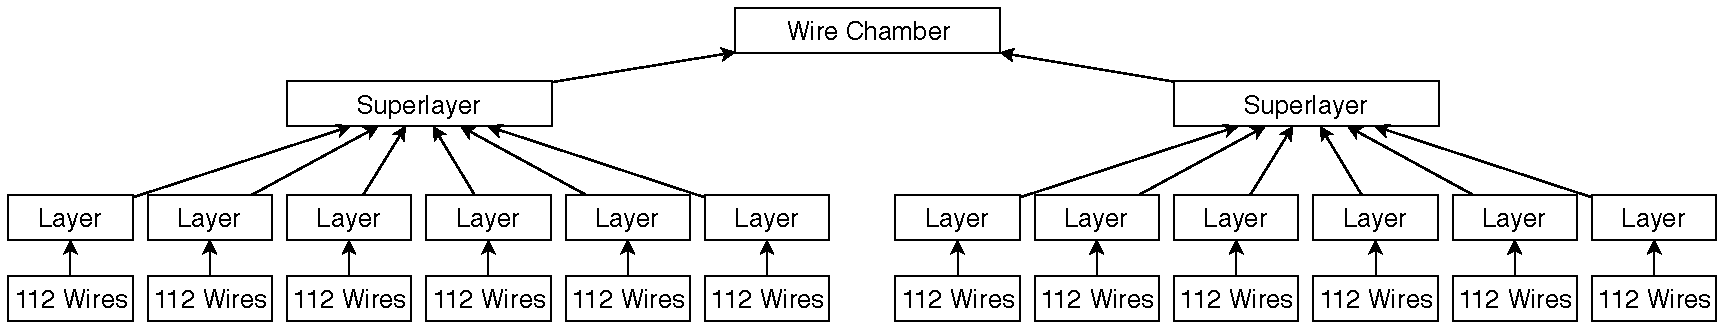
\includegraphics[width=\textwidth]{../figures/wire_chamber}
  \caption{The hierarchical structure of a single wire chamber.}
  \label{fig:wire-chamber}
\end{figure}

In order to gather as much information as possible on the particle
interactions, the 18 wire chambers are equally distributed across
three sectors within the drift chamber, the difference between the
sectors being their distance to the location of the electron beam hitting
the target. Sector one is located closest to the point of interest,
sector three is the furthest away.
